
%(BEGIN_QUESTION)
% Copyright 2012, Tony R. Kuphaldt, released under the Creative Commons Attribution License (v 1.0)
% This means you may do almost anything with this work of mine, so long as you give me proper credit

Examine this process trend showing the PV, SP, and Output of a loop controller:

$$\includegraphics[width=15.5cm]{i01924x01.eps}$$

Based on what you see here, determine the following:

\begin{itemize}
\item{} Whether this is an open-loop or a closed-loop response
\item{} Whether the controller is (or needs to be) {\it direct-acting} or {\it reverse-acting}
\item{} If possible, identify any problems with the field instrumentation
\item{} If possible, identify any problems with the controller PID tuning
\item{} Qualitatively identify the kind of PID tuning we will need for robust control
\end{itemize}

\underbar{file i01924}
%(END_QUESTION)





%(BEGIN_ANSWER)


%(END_ANSWER)





%(BEGIN_NOTES)

This is an {\it open-loop test}, based on the fact the output signal is square-wave stepping as it would when a human operator enters new values in manual mode.

\vskip 10pt

Since this is a manual-mode test, we know we are looking at the response of the {\it process}, not the {\it PID controller}.  Based on this test, we see the process has a direct response, which means the controller must be {\it reverse-acting} in order to have the negative feedback we need for stable control.

\vskip 10pt

The control valve seems to exhibit hysteresis: note how it fails to respond when the controller output is moved from 20\% to 25\%, and then again when the valve direction is reversed from 40\% to 35\%.  Failure to respond upon reversal of stimulus is the defining characteristic of any kind of hysteresis.

\vskip 10pt

We cannot tell if there are any tuning problems with the controller, because this trend does not show us the results in automatic mode (closed-loop).

\vskip 10pt

We can tell from the process response that this is a self-regulating process with about a half-minute of first-order lag combined with either a short second lag or dead time.  Consequently, we would expect to need integral action to avoid offset between PV and SP, plus some proportional action, and perhaps some derivative action as well to help counter the effects of the lags.


%INDEX% Control, PID tuning: step change (output) revealing valve hysteresis
%INDEX% Process troubleshooting: diagnosing problem via trend recording

%(END_NOTES)


